\section{Introduction}
\label{sec:intro}

A graph index and its search-budget policy jointly determine approximate nearest-neighbor search (ANNS) quality and cost. Rebuilding an HNSW or Vamana index changes traversal paths even when vectors and queries are unchanged; refreshing data also changes nearest-neighbor truth~\cite{malkov2020hnsw,subramanya2019diskann}. A retained budget is therefore versioned decision state, not inert configuration.

The relevant failure is query-level: $\rec@10<0.95$. Because recall is discrete, one missed neighbor is a failure. A 5\% risk limit asks that at least 95\% of queries return all ten neighbors. This differs from mean recall and exposes two effects that averages can hide: target queries unresolved even at the endpoint, and additional failure caused by a transferred action.

We organize the evidence around a deployment question: \emph{what target evidence is required before a budget policy can be reused?} First, graph-only transfer on unchanged SIFT-100K and Arxiv-Nomic-100K collections adds 17.17--23.60 percentage points of failure above target-specific references across hnswlib and Faiss. Second, after a 5\% data refresh, an unchanged recurring-query policy moves from 3.77\% to 6.69\% risk on SIFT and from 3.19\% to 7.24\% on Arxiv-Nomic. Third, fresh-build and fresh-query experiments test which recovery policies remain safe, fast, and robust.

\emph{Index-Conditioned Budget Audit} (ICBA) is the resulting decision contract. It declares the target index, workload, native action grid, failure event, permitted observations, candidate policy, target certificate, fallback, held-out evaluation, and acquisition ledger. This separation prevents four different claims---portability, qualification, serving gain, and lifecycle value---from being collapsed into one number.

We evaluate a hierarchy of recovery policies. A fixed action is the minimum-complexity baseline. Target-global calibration chooses one action using target labels. \emph{Target-calibrated pooling} (TCP) uses recurring-query histories and one target-selected global shift to retain query conditioning. A source-derived one-rung rule is a diagnostic bridge: it tests whether source evidence alone leaves useful slack, but it is not presumed superior to the simpler alternatives.

This hierarchy changes the interpretation of the recovery results. TCP retains 44.39\% and 29.86\% endpoint-relative mean-NDC reductions under the stricter completed decision. Relative to an equal-information target-global policy, its incremental mean benefit is clear on SIFT and unresolved with a worse p95 on Arxiv. In a separate preregistered panel with fresh insertion permutations and query roles, the frozen source-derived candidate qualifies every target decision and reduces measured wall time. The paired strong-baseline audit then finds that fixed-256 matches this candidate on SIFT and dominates it on Arxiv; target-global calibration is strongest when more target labels are available. The operational rule is therefore to deploy the least complex target-certified policy that meets the target SLA.

\begin{figure*}[t]
\centering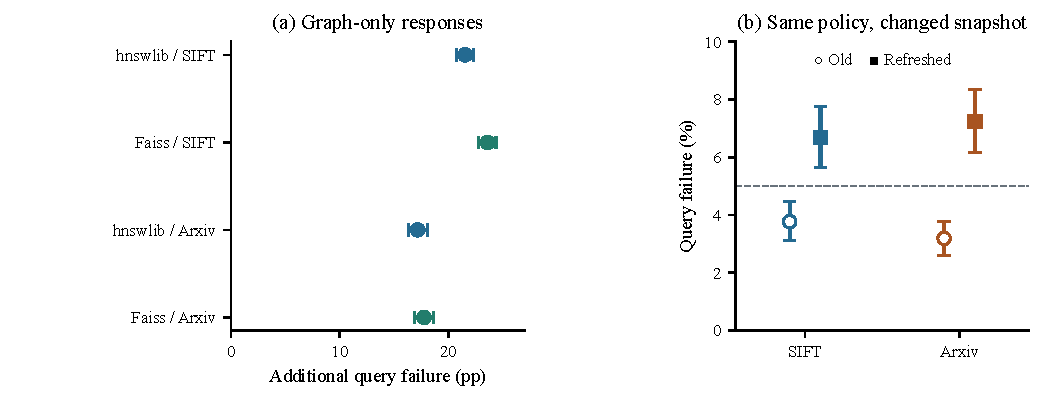
\includegraphics[width=\textwidth]{figures/overview.pdf}
\caption{Two failures that motivate ICBA. Left: graph-only transfer of retrospective first-passing actions, reported as additional failure above each target's reference. Right: one executable recurring-query policy replayed before and after a 5\% refresh. Intervals preserve shared query and target units.}
\label{fig:overview}
\Description{Four graph-only incremental-risk estimates are positive. In the refresh test, risk increases on both datasets and crosses five percent.}
\end{figure*}

\begin{table}[t]
\caption*{\textbf{Terms at a glance.} Tables shorten Arxiv-Nomic-100K to Arxiv.}
\small\begin{tabularx}{\linewidth}{@{}lX@{}}\toprule
Term & Meaning \\\midrule
ICBA & Audit contract for target portability and deployment.\\
TCP & Target-calibrated pooling for recurring profiled queries.\\
NDC & Number of distance calculations.\\
CP / UCB & Clopper--Pearson / upper confidence bound.\\
LOTO & Leave one target build out.\\
Endpoint & Largest registered native action.\\\bottomrule
\end{tabularx}
\end{table}

We make three contributions. First, we establish budget non-portability across graph-only rebuilds, data refresh, implementations, graph families, and 100K-to-1M scale while retaining each setting's estimand. Second, ICBA supplies a reusable protocol for separating response evidence, target qualification, completed execution, and information cost. Third, a preregistered recovery and baseline program identifies where complexity is warranted: target calibration is consistently valuable, TCP adds query-conditional value on SIFT, and a simple fixed action can dominate a source-tailored heuristic. The artifact independently regenerates the paper, validates the decision chain, and preserves all query-role boundaries.

The systems implication is direct: version the budget policy with its index and workload; qualify reuse on the target; and escalate from fixed to target-global to query-conditional policies only when the measured gain justifies their information cost.
